\documentclass[a0paper,landscape,final]{baposter}

\usepackage{times}
\usepackage{calc}
\usepackage{graphicx}
\usepackage{amsmath}
\usepackage{amssymb}
\usepackage{relsize}
\usepackage{multirow}
\usepackage{bm}
\usepackage{tkz-berge}
\usepackage[upright]{fourier}
\usepackage{bm}

\usepackage{graphicx}
\usepackage{multicol}

\usepackage{pgfbaselayers}
\pgfdeclarelayer{background}
\pgfdeclarelayer{foreground}
\pgfsetlayers{background,main,foreground}

\usepackage{helvet}
%\usepackage{bookman}
\usepackage{palatino}

\newcommand{\captionfont}{\footnotesize}

\selectcolormodel{cmyk}

\graphicspath{{images/}}

%%%%%%%%%%%%%%%%%%%%%%%%%%%%%%%%%%%%%%%%%%%%%%%%%%%%%%%%%%%%%%%%%%%%%%%%%%%%%%%%
%%%% Some math symbols used in the text
%%%%%%%%%%%%%%%%%%%%%%%%%%%%%%%%%%%%%%%%%%%%%%%%%%%%%%%%%%%%%%%%%%%%%%%%%%%%%%%%
% Format 
\newcommand{\Matrix}[1]{\begin{bmatrix} #1 \end{bmatrix}}
\newcommand{\Vector}[1]{\Matrix{#1}}
\newcommand*{\SET}[1]  {\ensuremath{\mathcal{#1}}}
\newcommand*{\MAT}[1]  {\ensuremath{\mathbf{#1}}}
\newcommand*{\VEC}[1]  {\ensuremath{\bm{#1}}}
\newcommand*{\CONST}[1]{\ensuremath{\mathit{#1}}}
\newcommand*{\norm}[1]{\mathopen\| #1 \mathclose\|}% use instead of $\|x\|$
\newcommand*{\abs}[1]{\mathopen| #1 \mathclose|}% use instead of $\|x\|$
\newcommand*{\absLR}[1]{\left| #1 \right|}% use instead of $\|x\|$

\def\norm#1{\mathopen\| #1 \mathclose\|}% use instead of $\|x\|$
\newcommand{\normLR}[1]{\left\| #1 \right\|}% use instead of $\|x\|$

\makeatletter
\newcommand*{\Tiny}{\@setfontsize\Tiny{12pt}{13pt}}
\makeatother

%%%%%%%%%%%%%%%%%%%%%%%%%%%%%%%%%%%%%%%%%%%%%%%%%%%%%%%%%%%%%%%%%%%%%%%%%%%%%%%%
% Multicol Settings
%%%%%%%%%%%%%%%%%%%%%%%%%%%%%%%%%%%%%%%%%%%%%%%%%%%%%%%%%%%%%%%%%%%%%%%%%%%%%%%%
\setlength{\columnsep}{0.7em}
\setlength{\columnseprule}{0mm}


%%%%%%%%%%%%%%%%%%%%%%%%%%%%%%%%%%%%%%%%%%%%%%%%%%%%%%%%%%%%%%%%%%%%%%%%%%%%%%%%
% Save space in lists. Use this after the opening of the list
%%%%%%%%%%%%%%%%%%%%%%%%%%%%%%%%%%%%%%%%%%%%%%%%%%%%%%%%%%%%%%%%%%%%%%%%%%%%%%%%
\newcommand{\compresslist}{%
\setlength{\itemsep}{1pt}%
\setlength{\parskip}{0pt}%
\setlength{\parsep}{0pt}%
}


%%%%%%%%%%%%%%%%%%%%%%%%%%%%%%%%%%%%%%%%%%%%%%%%%%%%%%%%%%%%%%%%%%%%%%%%%%%%%%
%%% Begin of Document
%%%%%%%%%%%%%%%%%%%%%%%%%%%%%%%%%%%%%%%%%%%%%%%%%%%%%%%%%%%%%%%%%%%%%%%%%%%%%%

\begin{document}

%%%%%%%%%%%%%%%%%%%%%%%%%%%%%%%%%%%%%%%%%%%%%%%%%%%%%%%%%%%%%%%%%%%%%%%%%%%%%%
%%% Here starts the poster
%%%---------------------------------------------------------------------------
%%% Format it to your taste with the options
%%%%%%%%%%%%%%%%%%%%%%%%%%%%%%%%%%%%%%%%%%%%%%%%%%%%%%%%%%%%%%%%%%%%%%%%%%%%%%
\typeout{Poster Starts}
\background{
  \begin{tikzpicture}[remember picture,overlay]%
    \draw (current page.north west)+(-2em,-0em) node[anchor=north west] {\hspace{-2em}
\includegraphics[height=1.1\textheight]{silhouettes_background}};
  \end{tikzpicture}%
}
\definecolor{silver}{cmyk}{0,0,0,0.3}
\definecolor{yellow}{cmyk}{0,0,0.9,0.0}
\definecolor{reddishyellow}{cmyk}{0,0.22,1.0,0.0}
\definecolor{black}{cmyk}{0,0,0.0,1.0}
\definecolor{darkYellow}{cmyk}{0,0,1.0,0.5}
\definecolor{darkSilver}{cmyk}{0,0,0,0.1}

\definecolor{lightyellow}{cmyk}{0,0,0.3,0.0}
\definecolor{lighteryellow}{cmyk}{0,0,0.1,0.0}
\definecolor{lighteryellow}{cmyk}{0,0,0.1,0.0}
\definecolor{lightestyellow}{cmyk}{0,0,0.05,0.0}
\begin{poster}{
  % Show grid to help with alignment
  grid=false,
  % Column spacing
  colspacing=1em,
  % Color style
  bgColorOne=lighteryellow,
  bgColorTwo=lightestyellow,
  borderColor=reddishyellow,
  headerColorOne=lightyellow,
  headerColorTwo=silver,
  headerFontColor=black,
  boxColorOne=lightestyellow,
  boxColorTwo=lightestyellow,
  % Format of textbox
  textborder=roundedleft,
  % Format of text header
  eyecatcher=false,
  headerborder=open,
  headerheight=0.08\textheight,
  headershape=roundedright,
  headershade=plain,
  headerfont=\Tiny, %\textsf, %Sans Serif
  boxshade=plain,
%  background=shade-tb,
  background=plain,
  linewidth=1pt
  }
  % Eye Catcher
  {} % No eye catcher for this poster. If an eye catcher is present, the title is centered between eye-catcher and logo.
  % Title
  {\sf %Sans Serif
  %\bf% Serif
  \vspace{0.5em}
  Unsupervised Feature Learning for Object Classification
  \vspace{0.2em}
  }
  % Authors
  {\sf %Sans Serif
  % Serif
  Laxman Dhulipala, Harry Gifford, Wangzi He\hspace{3em}
  \{ldhulipa, hgifford, wangzih\}@andrew.cmu.edu\hspace{3em}
  }
  % University logo
  {{\begin{minipage}{25em}
    \hfill
%    
\includegraphics[height=2em]{msrlogo}
%    
\includegraphics[height=5.5em]{logo}
%     
\includegraphics[width=10em]{cmu_seal}
  \end{minipage}}
  }

  \tikzstyle{light shaded}=[top color=baposterBGtwo!30!white,bottom color=baposterBGone!30!white,shading=axis,shading angle=30]

  % Width of left inset image
     \newlength{\leftimgwidth}
     \setlength{\leftimgwidth}{0.78em+8.0em}

%%%%%%%%%%%%%%%%%%%%%%%%%%%%%%%%%%%%%%%%%%%%%%%%%%%%%%%%%%%%%%%%%%%%%%%%%%%%%%
%%% Now define the boxes that make up the poster
%%%---------------------------------------------------------------------------
%%% Each box has a name and can be placed absolutely or relatively.
%%% The only inconvenience is that you can only specify a relative position 
%%% towards an already declared box. So if you have a box attached to the 
%%% bottom, one to the top and a third one which should be in between, you 
%%% have to specify the top and bottom boxes before you specify the middle 
%%% box.
%%%%%%%%%%%%%%%%%%%%%%%%%%%%%%%%%%%%%%%%%%%%%%%%%%%%%%%%%%%%%%%%%%%%%%%%%%%%%%
    %
    % A coloured circle useful as a bullet with an adjustably strong filling
    \newcommand{\colouredcircle}[1]{%
      \tikz{\useasboundingbox (-0.2em,-0.32em) rectangle(0.2em,0.32em); \draw[draw=black,fill=baposterBGone!80!black!#1!white,line width=0.03em] (0,0) circle(0.18em);}}

%%%%%%%%%%%%%%%%%%%%%%%%%%%%%%%%%%%%%%%%%%%%%%%%%%%%%%%%%%%%%%%%%%%%%%%%%%%%%%
  \headerbox{Contribution}{name=contribution,column=0,row=0}{
%%%%%%%%%%%%%%%%%%%%%%%%%%%%%%%%%%%%%%%%%%%%%%%%%%%%%%%%%%%%%%%%%%%%%%%%%%%%%%
   {}
   
   We implement an unsupervised method for learning features from images,
   which are then used for image classification. Our method is robust, and
   we experimentally show its performance on the CIFAR-10 dataset, a standard
   dataset in the machine learning community. We implement and describe a 
   feature-learning pipeline, which can be recursively applied in order to learn
   successively more general features. 
 }

%%%%%%%%%%%%%%%%%%%%%%%%%%%%%%%%%%%%%%%%%%%%%%%%%%%%%%%%%%%%%%%%%%%%%%%%%%%%%%
  \headerbox{Model}{name=model,column=0,below=contribution}{
%%%%%%%%%%%%%%%%%%%%%%%%%%%%%%%%%%%%%%%%%%%%%%%%%%%%%%%%%%%%%%%%%%%%%%%%%%%%%%
    The Model was learnt from 175 subjects. We used one neutral expression scan
    per identity and 50 expression scans of a subset of the subjects. 

    The identity model is a linear model build from the neutral scans.
    \begin{align}
      \VEC f&=\VEC\mu + \MAT M_n\VEC\alpha_n\qquad.
    \end{align}
    For each of the 50 expression scans, we calculated an expression vector as
    the difference between the expression scan and the corresponding neutral
    scan of that subject.  This data is already mode-centered, if we regard the
    neutral expression as the natural mode of expression data. From these offset
    vectors an additional expression matrix $\MAT M_e$ was calculated, such that the complete linear Model is
    \begin{align}
      \VEC f&=\VEC\mu + \MAT M_n\VEC\alpha_n + \MAT M_e\VEC\alpha_e
    \end{align}
    The assumption here is, that the face and expression space are linearly
    independent, such that each face is represented by a unique set of
    coefficients.  
  }

%%%%%%%%%%%%%%%%%%%%%%%%%%%%%%%%%%%%%%%%%%%%%%%%%%%%%%%%%%%%%%%%%%%%%%%%%%%%%%
  \headerbox{Fitting}{name=fitting,column=0,below=model}{
%%%%%%%%%%%%%%%%%%%%%%%%%%%%%%%%%%%%%%%%%%%%%%%%%%%%%%%%%%%%%%%%%%%%%%%%%%%%%%
    A Robust Nonrigid ICP method was used to fit the model to the data.
    Robustness was achieved by iteratively reweighting the correspondences and
    using hard compatability test for the closest points.

    Fitting was initialized by a simple nose detector and proceeded fully
    automatic.
  }

%%%%%%%%%%%%%%%%%%%%%%%%%%%%%%%%%%%%%%%%%%%%%%%%%%%%%%%%%%%%%%%%%%%%%%%%%%%%%%
  \headerbox{Distance Measure}{name=measure,column=0,below=fitting,above=bottom}{
%%%%%%%%%%%%%%%%%%%%%%%%%%%%%%%%%%%%%%%%%%%%%%%%%%%%%%%%%%%%%%%%%%%%%%%%%%%%%%
   The Mahalanobis angle between the identity coefficients $\VEC{\alpha_{n}}$
   was used for classification.
  }

%%%%%%%%%%%%%%%%%%%%%%%%%%%%%%%%%%%%%%%%%%%%%%%%%%%%%%%%%%%%%%%%%%%%%%%%%%%%%%
  \headerbox{Expression Neutralization}{name=results neutralization,column=1,row=0}{
%%%%%%%%%%%%%%%%%%%%%%%%%%%%%%%%%%%%%%%%%%%%%%%%%%%%%%%%%%%%%%%%%%%%%%%%%%%%%%
  \begin{tabular}{@{}c@{ }c@{ }c@{ }c@{}@{ }@{ }c@{ }c@{ }c@{ }c@{ }}
    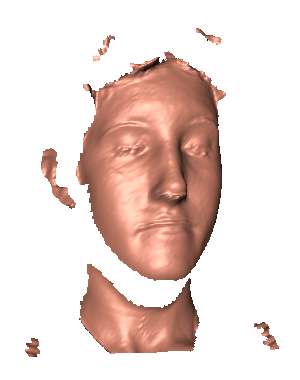
\includegraphics[height=0.42\linewidth]{16_1_tgt}&
    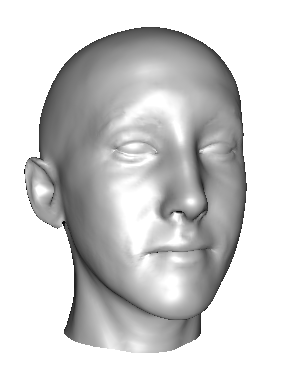
\includegraphics[height=0.42\linewidth]{16_1_expression}&
    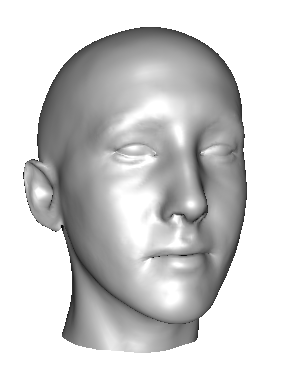
\includegraphics[height=0.42\linewidth]{16_1_neutral}\\[-0.8em]
    \smaller a) Target & \smaller b) Fit & \smaller c) Normalized\\[0.8em]
    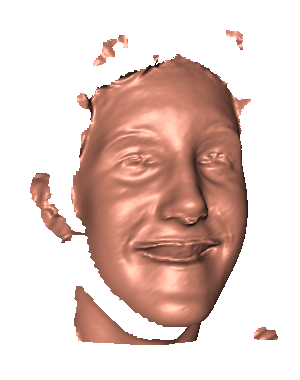
\includegraphics[height=0.42\linewidth]{16_6_tgt}&
    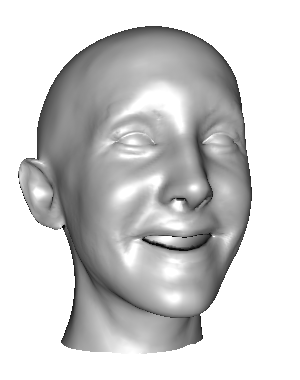
\includegraphics[height=0.42\linewidth]{16_6_expression}&
    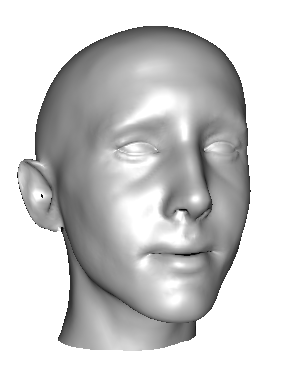
\includegraphics[height=0.42\linewidth]{16_6_neutral}\\[-0.8em]
    \smaller a) Target & \smaller b) Fit & \smaller c) Normalized
  \end{tabular}
  Expression normalisation for two scans of the same individual.  
  The robust fitting gives a good estimate (b) of the true face surface given
  the noisy measurement (a). It fills in holes and removes artifacts using
  prior knowledge from the face model. The pose and expression normalized faces
  (c) are used for face recognition.
  }
%%%%%%%%%%%%%%%%%%%%%%%%%%%%%%%%%%%%%%%%%%%%%%%%%%%%%%%%%%%%%%%%%%%%%%%%%%%%%%
  \headerbox{Robustness}{name=robustness,column=1,below=results neutralization,span=1,above=bottom}{
%%%%%%%%%%%%%%%%%%%%%%%%%%%%%%%%%%%%%%%%%%%%%%%%%%%%%%%%%%%%%%%%%%%%%%%%%%%%%%
  \begin{tabular}{@{}c@{ }c@{ }c@{ }c@{}}
    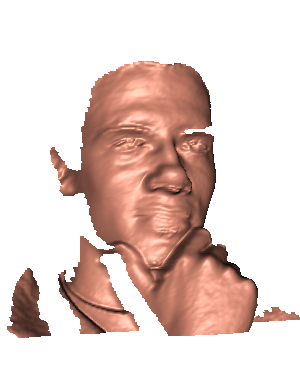
\includegraphics[height=0.42\linewidth]{56_4_tgt}&
    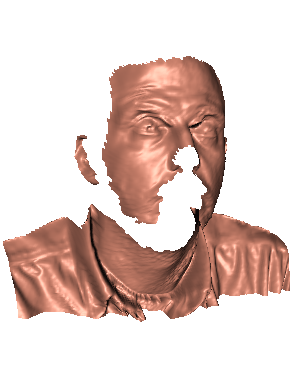
\includegraphics[height=0.42\linewidth]{23_2_tgt}&
    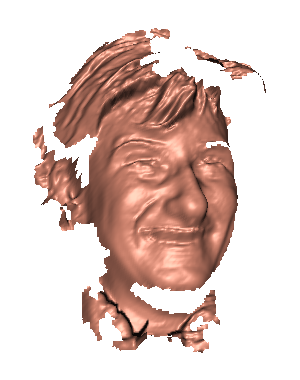
\includegraphics[height=0.42\linewidth]{5_6_tgt}\\[-0.8em]
                       & \smaller a) Targets & \\[0.8em]
    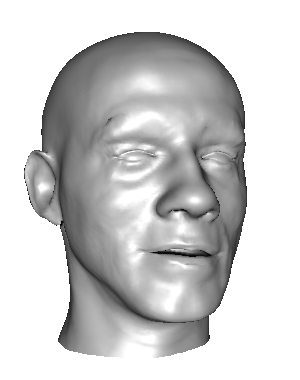
\includegraphics[height=0.42\linewidth]{56_4_expression}&
    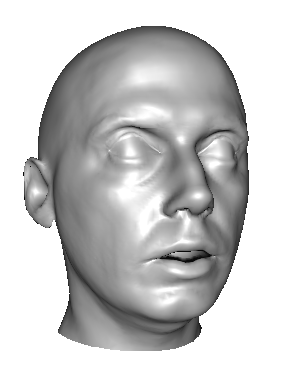
\includegraphics[height=0.42\linewidth]{23_2_expression}& 
    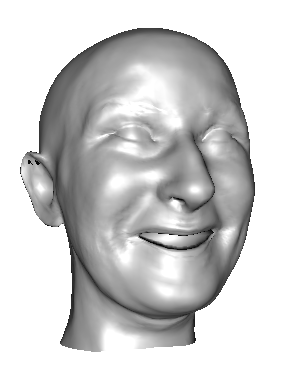
\includegraphics[height=0.42\linewidth]{5_6_expression}\\[-0.8em]
                    & \smaller b) Fits & 
  \end{tabular}
  The reconstruction (b) is robust against scans (a) with artifacts, noise, and
  holes.
  }
%%%%%%%%%%%%%%%%%%%%%%%%%%%%%%%%%%%%%%%%%%%%%%%%%%%%%%%%%%%%%%%%%%%%%%%%%%%%%%
  \headerbox{Results}{name=results,column=2,span=2,row=0}{
%%%%%%%%%%%%%%%%%%%%%%%%%%%%%%%%%%%%%%%%%%%%%%%%%%%%%%%%%%%%%%%%%%%%%%%%%%%%%%
      \begin{multicols}{2}
        The method was evaluated on the GavabDB expression dataset which
        contains 427 Scans, with 3 neutral scans and 4 expression scans per ID.
        To test the impact of expression invariance on neutral data we used the
        UND Dataset from the Face Recognition Great Vendor Test, which contains
        953 neutral scans with one to eight scans per subject.
      \end{multicols}\vspace{-1em}
%      \mbox{\hspace{0.3\linewidth}\rule{0.4\linewidth}{1pt}\hspace{0.3\linewidth}}\\
%      \begin{tabular}{cc}
%        \hspace{0.5em}\scalebox{0.74}{\input{shrec_MNCG}} &
%        \hspace{0.5em}\scalebox{0.74}{\input{und_MNCG}}
%      \end{tabular}\\
        {Expression neutralization improves results on the expression dataset
        without decreasing the accuracy on the neutral testset. Plotted is the
        ratio of correct answers to  the number of possible correct answers.
        %Note the different scales for the two graphs.
        %Our approach has a high accuracy on the neutral (UND) dataset.
        }
%      \end{multicols}\vspace{-1em}
      \\\mbox{\hspace{0.3\linewidth}\rule{0.4\linewidth}{1pt}\hspace{0.3\linewidth}}\\
%      \begin{tabular}{cc}
%        \hspace{0.5em}\scalebox{0.74}{\input{shrec_PR}} &
%        \hspace{0.5em}\scalebox{0.74}{\input{und_PR}}
%      \end{tabular}\\
%      \begin{multicols}{2}
        {Plotted are precision and recall for different retrieval depths. The lower
        precision of the UND database is due to the fact that some queries have no
        correct answers.}
%      \end{multicols}\vspace{-1em}
%      \\\mbox{\hspace{0.3\linewidth}\rule{0.4\linewidth}{1pt}\hspace{0.3\linewidth}}\\
%%      \begin{tabular}{cc}
%%        \hspace{0.5em}\scalebox{0.74}{\input{shrec_FARFRR}} &
%%        \hspace{0.5em}\scalebox{0.74}{\input{und_FARFRR}}
%%      \end{tabular}\\
%%      \begin{multicols}{2}
%        {Impostor detection is reliable, as the minimum distance to a match
%        is smaller than the minimum distance to a nonmatch. }
%      \end{multicols}
\\
  }%
%%%%%%%%%%%%%%%%%%%%%%%%%%%%%%%%%%%%%%%%%%%%%%%%%%%%%%%%%%%%%%%%%%%%%%%%%%%%%%
  \headerbox{Open Questions}{name=questions,column=2,span=1,above=bottom,below=results}{
%%%%%%%%%%%%%%%%%%%%%%%%%%%%%%%%%%%%%%%%%%%%%%%%%%%%%%%%%%%%%%%%%%%%%%%%%%%%%%
    While the expression and identity space are linearly independent, there is
    some expression left in the identity model. This is because a ``neutral''
    face is interpreted differently by the subjects. We investigate the
    possibilty to build an identity/expression separated model without using
    the data labelling, based on a measure of independence.
  }%
%%%%%%%%%%%%%%%%%%%%%%%%%%%%%%%%%%%%%%%%%%%%%%%%%%%%%%%%%%%%%%%%%%%%%%%%%%%%%%
  \headerbox{Funding}{name=funding,column=3,span=1,above=bottom}{
%%%%%%%%%%%%%%%%%%%%%%%%%%%%%%%%%%%%%%%%%%%%%%%%%%%%%%%%%%%%%%%%%%%%%%%%%%%%%%
  \smaller 
  This work was supported in part by Microsoft Research through the European PhD Scholarship Programme.
  }%
%%%%%%%%%%%%%%%%%%%%%%%%%%%%%%%%%%%%%%%%%%%%%%%%%%%%%%%%%%%%%%%%%%%%%%%%%%%%%%
  \headerbox{References}{name=references,column=3,above=funding,below=results}{
%%%%%%%%%%%%%%%%%%%%%%%%%%%%%%%%%%%%%%%%%%%%%%%%%%%%%%%%%%%%%%%%%%%%%%%%%%%%%%
\smaller
\bibliographystyle{abbrv}
\bibliography{ref}

%    \smaller
%    \vspace{-0.4em}
%    \bibliographystyle{ieee}
%    \renewcommand{\section}[2]{\vskip 0.05em}
%      \begin{thebibliography}{1}\itemsep=-0.01em
%      \setlength{\baselineskip}{0.4em}
%      \bibitem{amberg07:nonrigid}
%        B.~Amberg, S.~Romdhani, T. Vetter.
%        \newblock {O}ptimal {S}tep {N}onrigid {ICP} {A}lgorithms for {S}urface {R}egistration
%        \newblock In {\em CVPR 2007}
%      \bibitem{amberg08:recognition}
%        B.~Amberg, R.~Knothe, T. Vetter.
%        \newblock Expression Invariant Face Recognition with a 3D Morphable Model
%        \newblock In {\em AFGR 2008}
%      \end{thebibliography}
  }%
\end{poster}%
%
\end{document}
